\documentclass[12pt,letterpaper]{hmcpset}
\usepackage[margin=1in]{geometry}
\usepackage{graphicx}
\usepackage{amsmath}

% info for header block in upper right hand corner
\name{ }
\class{Math 45 - Section --- \hspace{20pt}}
\assignment{HW 3}
\duedate{Tuesday, March 22, 2016}

\newcommand{\pn}[1]{\left( #1 \right)}
\newcommand{\abs}[1]{\left| #1 \right|}
\newcommand{\bk}[1]{\left[ #1 \right]}

\newcommand{\vb}{\mathbf{v}}
\newcommand{\ub}{\mathbf{u}}
\renewcommand{\labelenumi}{{(\alph{enumi})}}

\begin{document}

\problemlist{1, 2, 3, 4, 5, 6, 7}

% 1 %
\begin{problem}[1]
Which of these differential equations is separable? For those equations that are separable,
separate them. You don’t have to solve any of these equations.
\begin{enumerate}
	\item $\displaystyle{\frac{dy}{dx} = \frac{e^{x+y}}{xy}}$
	\item $C'(q) = q^2+2qC(q)$
	\item $\dot{z} = \omega$, $\omega$ is constant.
	\item $\displaystyle{y' = \ln\left({\frac{x}{y}}\right)}$
	\item $x' + 2 = tx-2x+t$
\end{enumerate}
\end{problem}

\begin{solution}
  \vfill
\end{solution}
\newpage

% 2 %
\begin{problem}[2]
  \begin{enumerate}
  	\item Find the general solution to the equation 
  	
  	$$\frac{dy}{dt} = \frac{4 \sin(2t)}{y}$$
  	
  	Your answer should be an explicit function $y(t)$ with two branches. 
  	 
  	\item Now impose the initial condition $y(0)=1$.  What is the solution to the DE that satisfies this initial condition?  
  	
  	\item What is the largest $t$-interval on which the solution is defined?\\
  	\textbf{Note:} You may be interested to look at the last two slides of Lecture 1, posted on Sakai, which give a bit more information on how to find the interval (domain) of validity for the solution to a DE.
  	
  \end{enumerate}
\end{problem}

\begin{solution}
  \vfill
\end{solution}
\newpage

% 3 %
\begin{problem}[3]
  Find all solutions to the ODE
  
  $$yy' = (1-y^2)\sin x. $$
  
  Your answer will be an implicit function of $y$ and $x$.  Make sure you don't ``lose'' any solutions along the way.
\end{problem}

\begin{solution}
  \vfill
\end{solution}
\newpage

\begin{problem}[4]
Using the integrating factor method find the general solution to the following differential equations.
\begin{enumerate}
	\item $2y' + 3y = e^{4t}$
	\item $y' + ty = 5t$
\end{enumerate}
\end{problem}

\begin{solution}
  \vfill
\end{solution}
\newpage

\begin{problem}[5]
	Examine Student X's work on the following problem.  What did the student do correctly?  What mistake(s) did the student make?  What is a more correct response to the problem, and what would you say to help the student understand how to correctly complete the problem?
	
	\begin{center}
		\parbox[c]{5.5in}{Determine the solution to the IVP $y'=5-ty$ with $y(0)=1$.\\
				
		\centering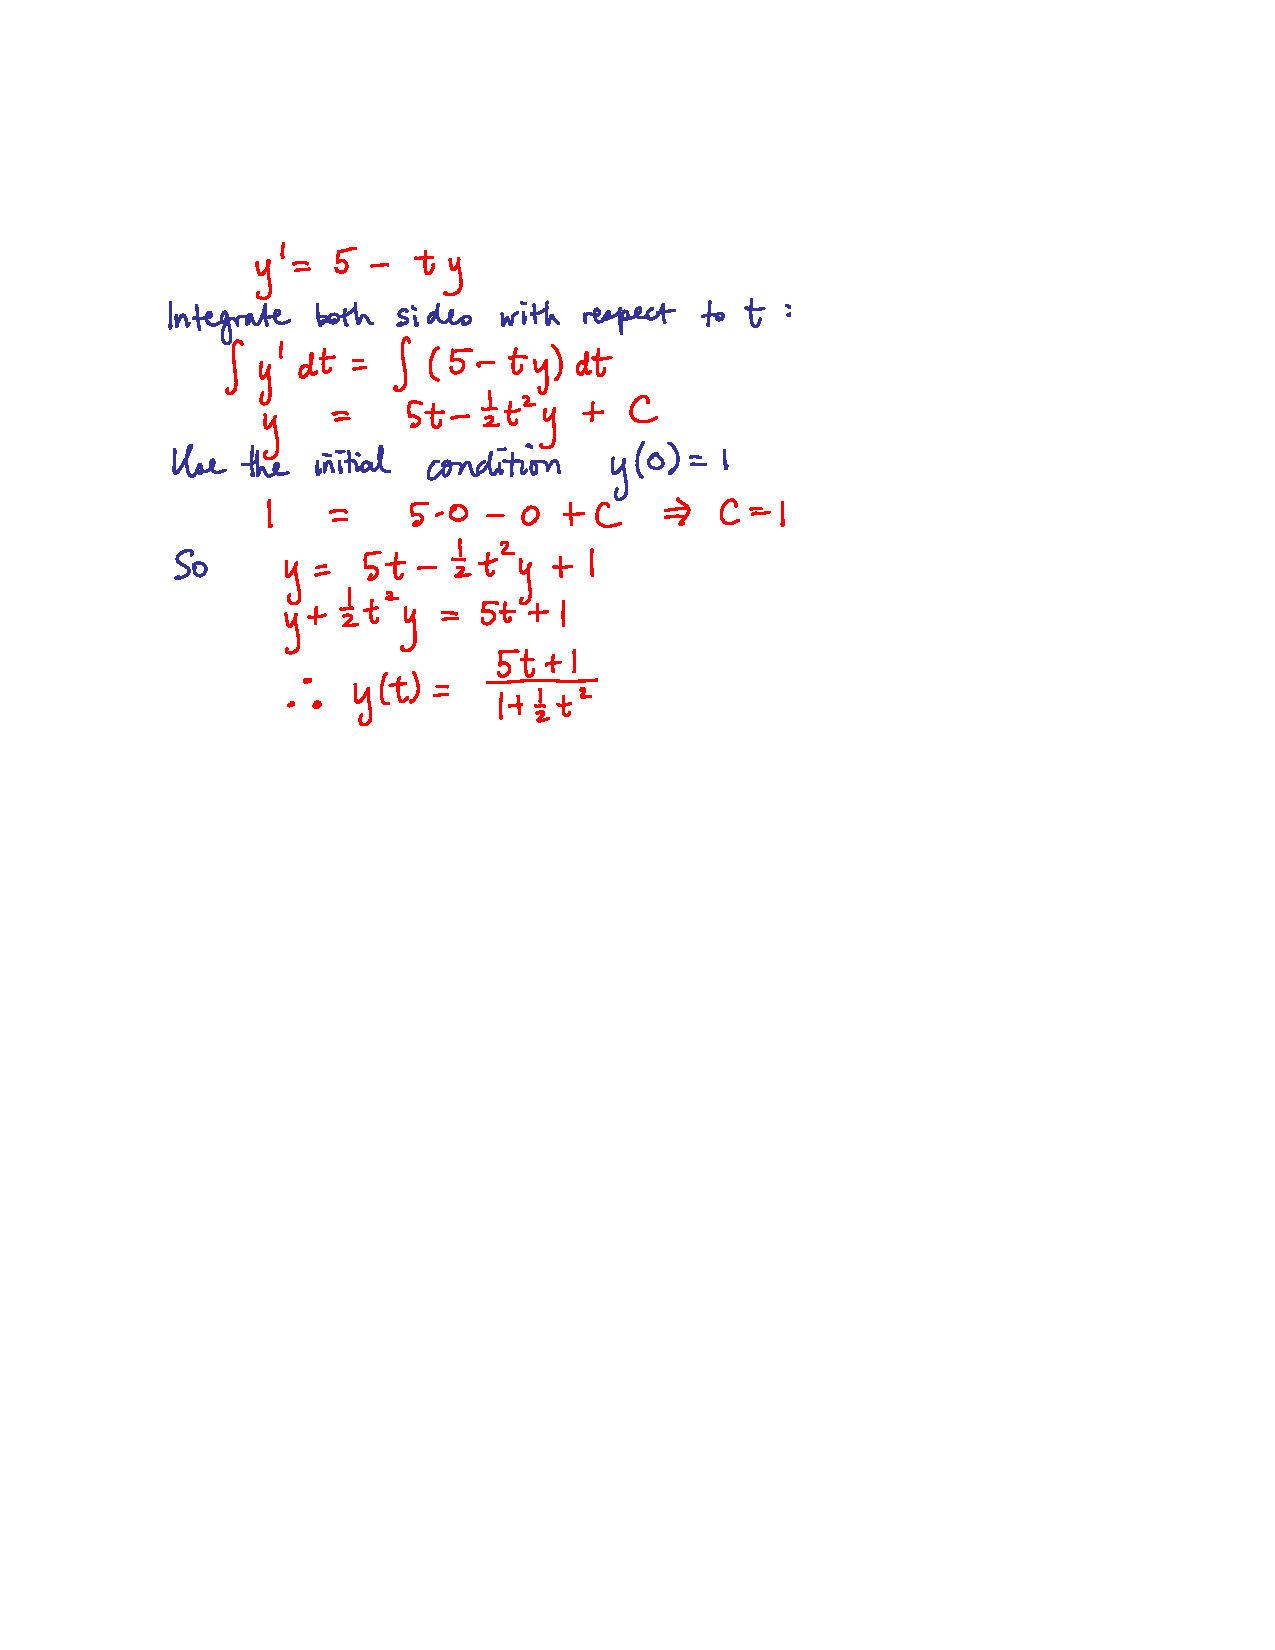
\includegraphics[width=3.5in,keepaspectratio=true]{img/mar_22_5}}
	\end{center}
\end{problem}

\begin{solution}
	\vfill
\end{solution}
\newpage

\begin{problem}[6]
  You can solve $y''=x\left(y'\right)^2$ with the initial conditions $y'(0) = -2$ and $y(0) = 0$, using a change of variables combined with  separation of variables.  This simple example illustrates a technique that can be applied to harder problems.  Here's the idea:  
  \begin{itemize}
  	\item First define a new variable, $w=y'$.  
  	\item Rewrite the original DE in terms of $w$ to get a separable ODE. 
  	\item Solve this equation to find $w(x)$ (Note: You may want to use one of the initial condition at this point).  
  	\item Substitute the answer you get for $w(x)$ into $w=y'$ and solve for $y$.  
  	\item Show that your solution satisfies the original DE and initial conditions.
  \end{itemize}
\end{problem}

\begin{solution}
  \vfill
\end{solution}
\newpage

\begin{problem}[7]
  Satellite dishes, radar antennae and microwave relays are designed so that they collect and focus an incoming signal into a single point (see Figure 1).  In this problem you will use differential equations to determine the dish shape that imparts this focusing property.  For simplicity assume that we are working with a cross-section of the dish, represented by a curve $y(x)$.  Incoming waves traveling parallel to the $y$-axis reflect off the dish according to the {\it law of reflection}:  the angle of incidence is equal to the angle of reflection.
  	\parbox[c]{6in}{
  	\centering
  	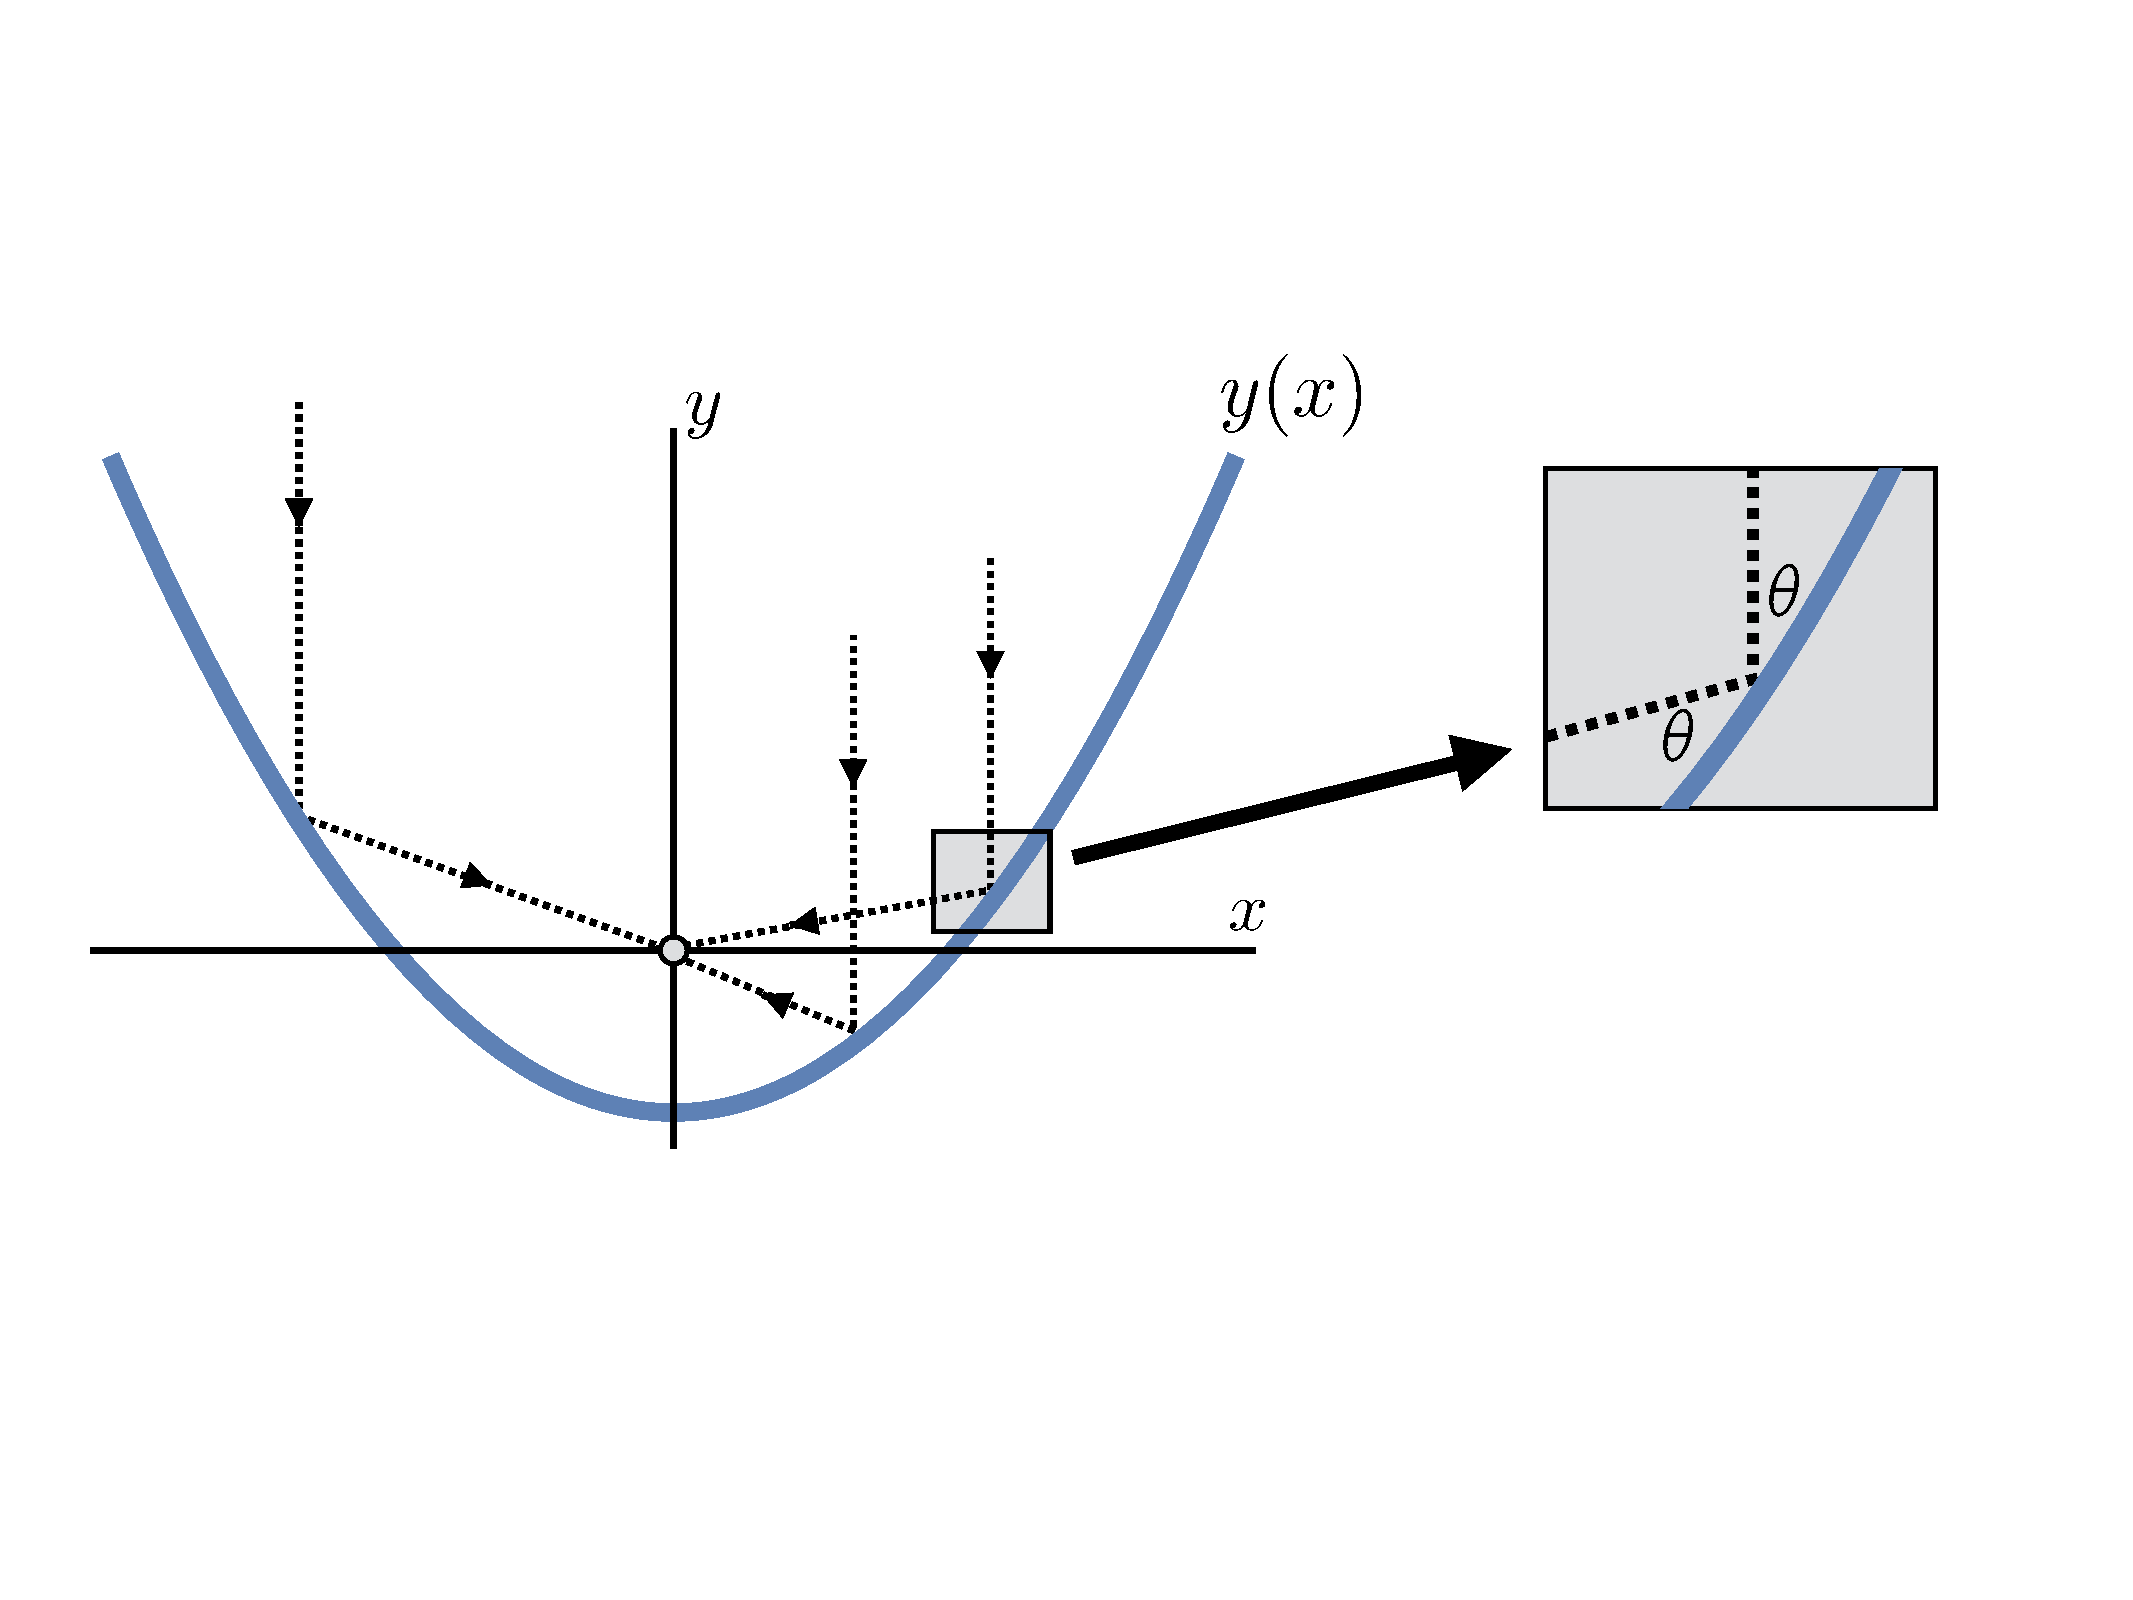
\includegraphics[width=3.4in]{img/mar_22_7}\\
  	Figure 1: A cross-section of a satellite dish, with law of reflection illustrated.}  
  \begin{enumerate}
  	\item For convenience, let's place the focus point at the origin. Consider the triangle formed by the tangent line to the dish at $(x,y)$, the reflected ray, and the $y$-axis, as shown on the left in Figure 2. Explain why this triangle must be isosceles.
  	  \parbox[c]{6in}{
  	  	\centering
  		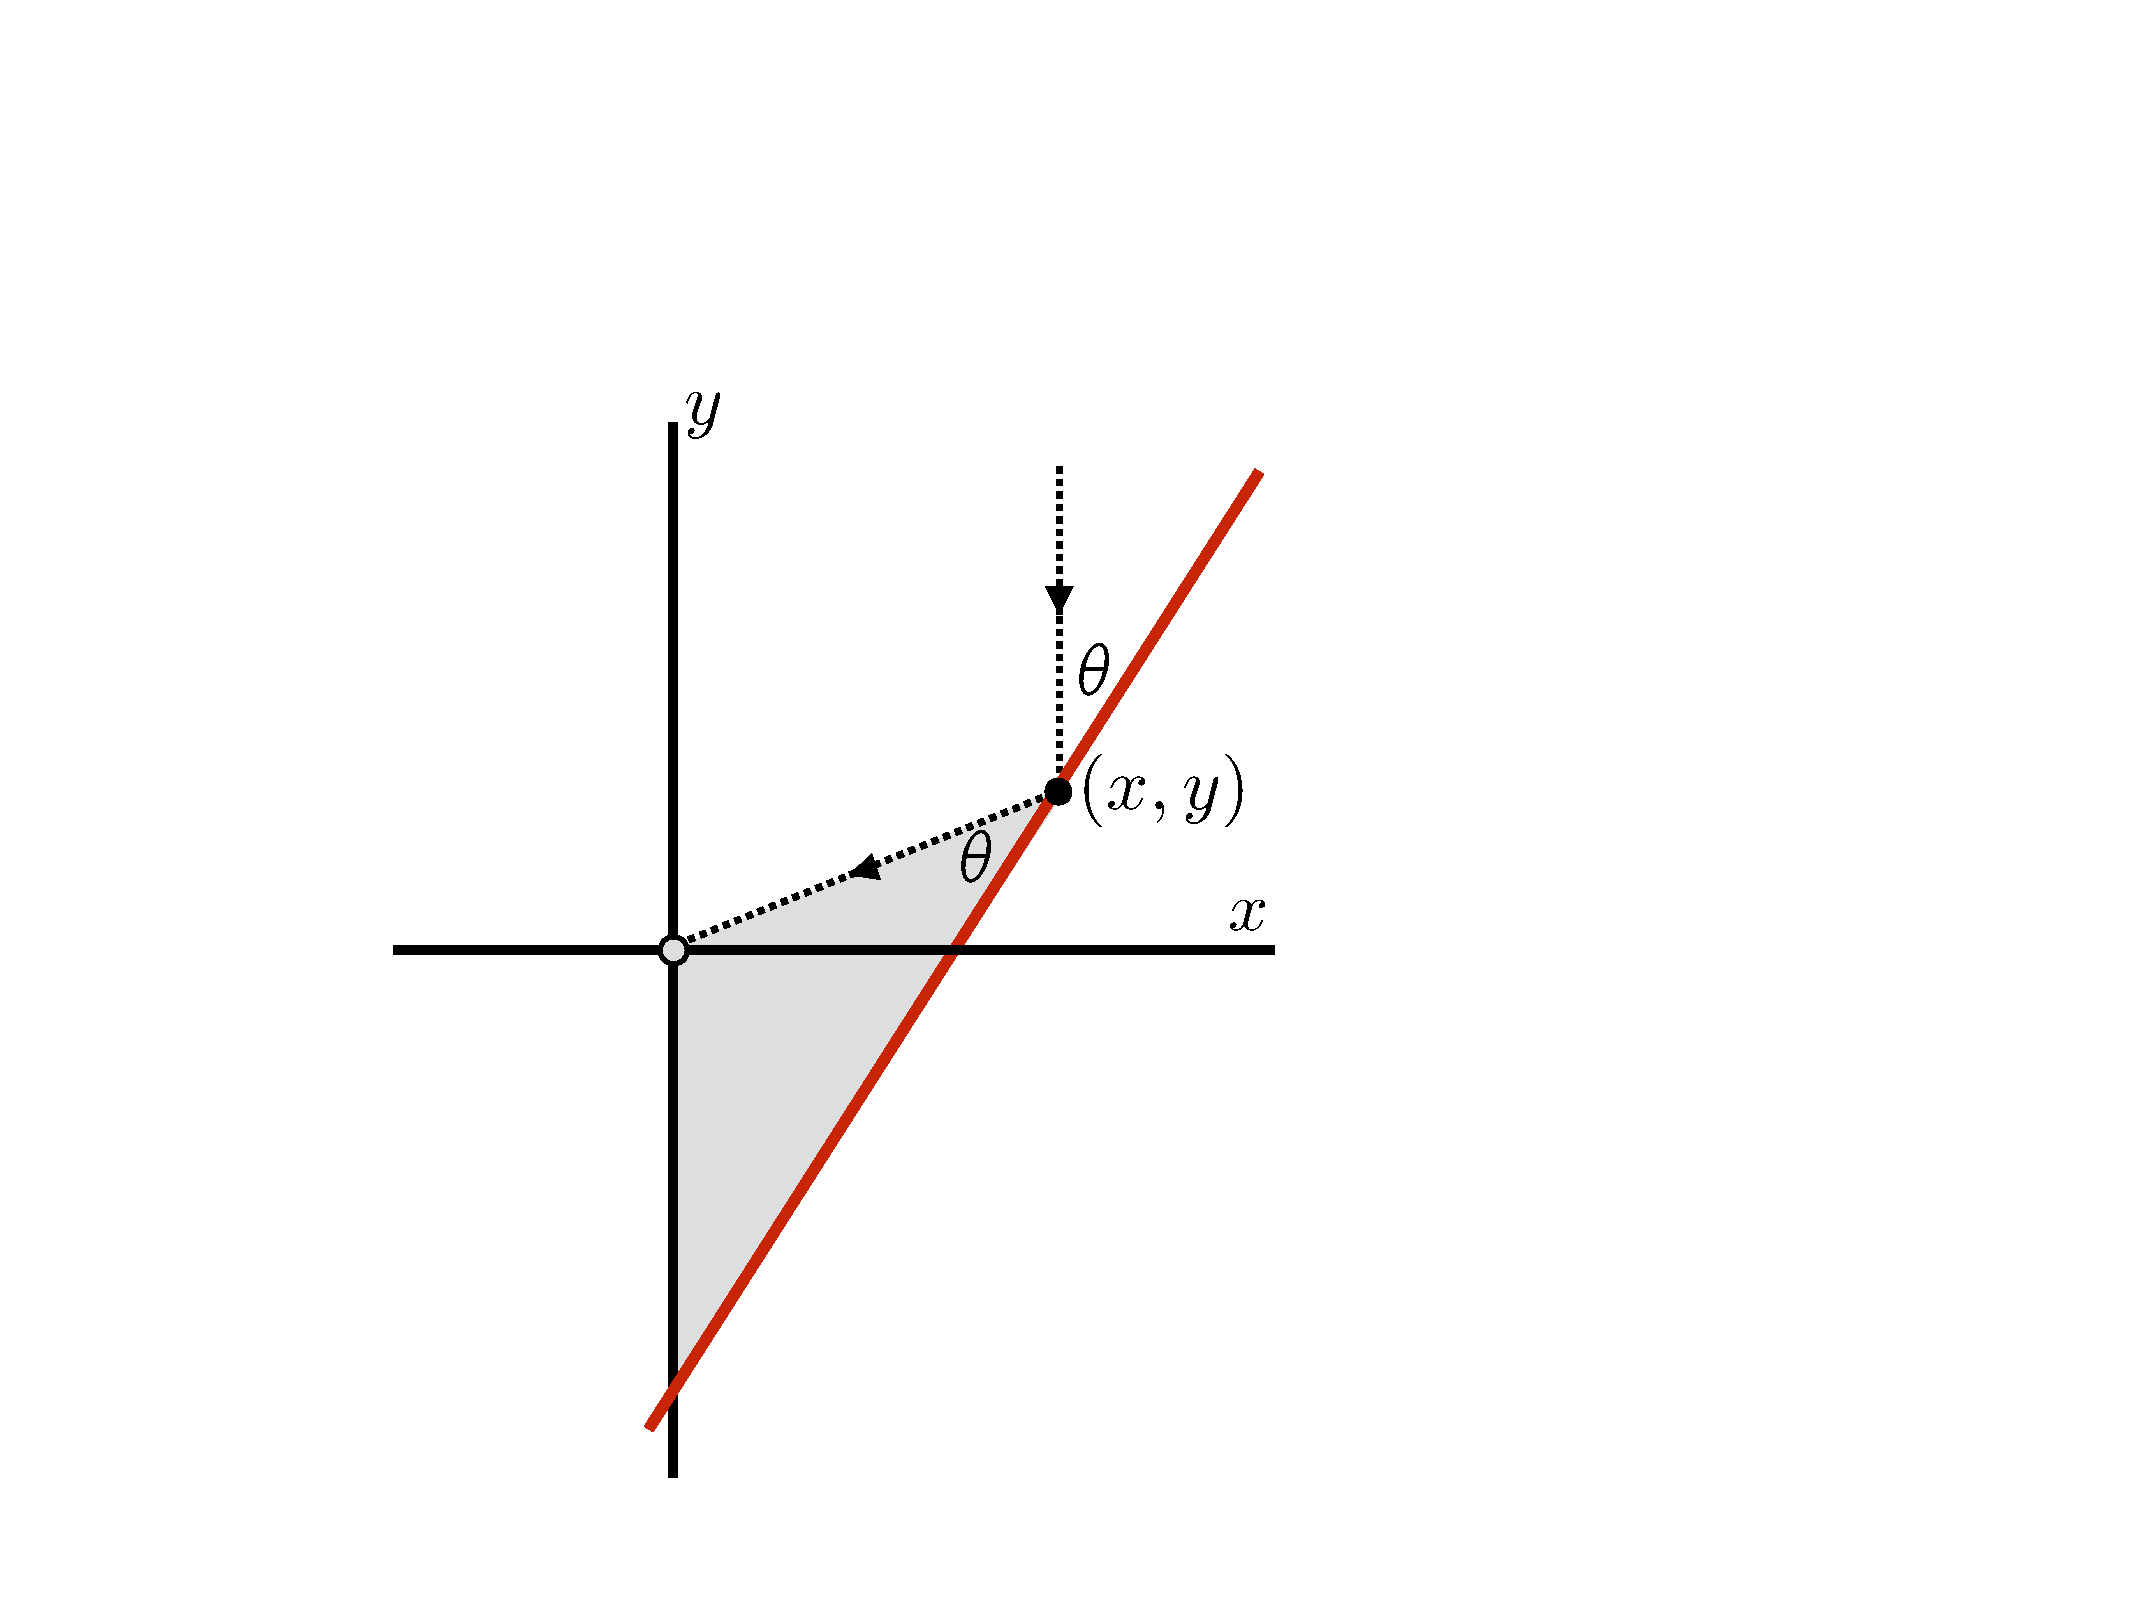
\includegraphics[width=1.7in]{img/mar_22_7a1}\qquad\qquad 
  		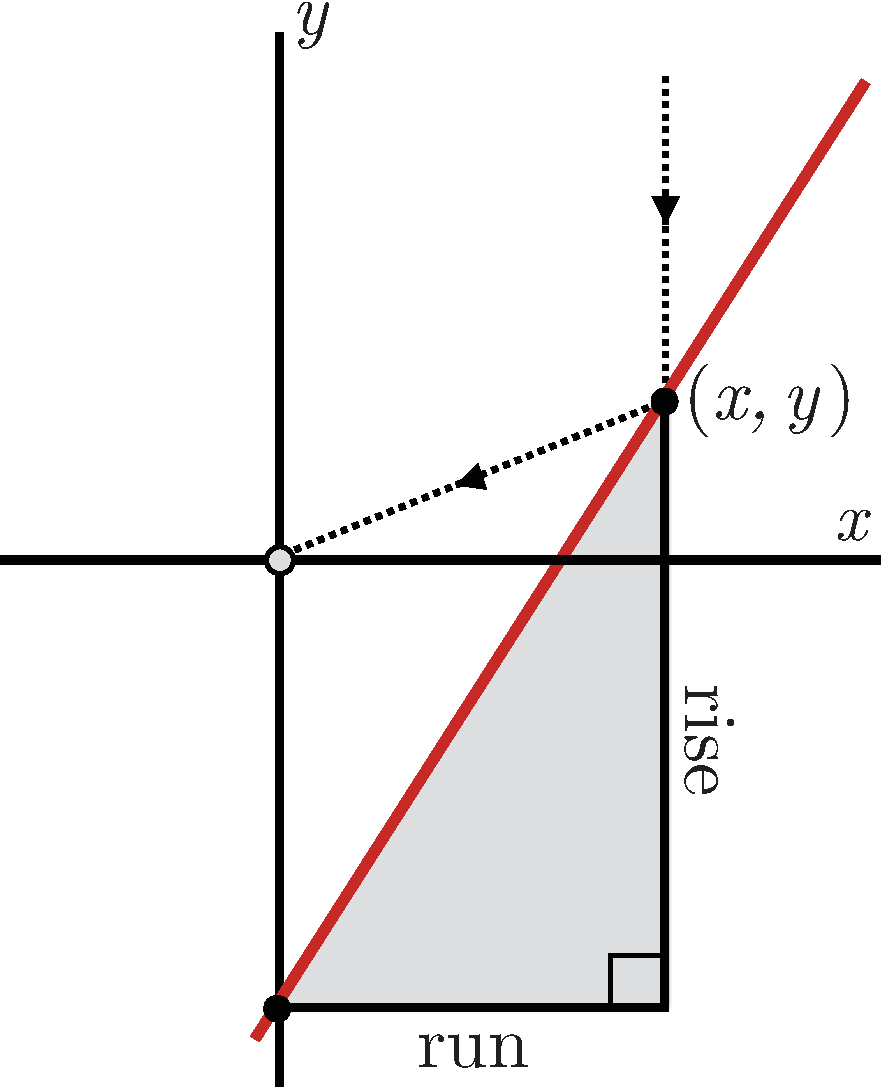
\includegraphics[width=1.6in]{img/mar_22_7a2}\\ Figure 2: Two triangles to help you derive the differential equation.}
  \begin{enumerate}
    \setcounter{enumi}{1}
    \item Based on your work on part (a), show that if the dish focuses
    incoming rays into a single point, then the curve of the dish,
    $y(x)$, must satisfy the differential equation
    \[
    \frac{dy}{dx} = \frac{y+\sqrt{x^2+y^2}}{x}.
    \]
    Hint:  Think of $dy/dx$ above as a slope, which is calculated as the ``rise over run'' in the right triangle on the right in Figure 2.
    
    \item  Using the substitution $y(x) = xz(x)$, show that the differential equation found in part (b) can be transformed into the equation
    \[
    z^\prime = \frac{\sqrt{1+z^2}}{x}.
    \]
    You may assume that $x>0$ throughout your computation.
    
    \item Solve the ODE from part (c) and determine the shape of the dish, $y(x)$.
  \end{enumerate}
  \end{enumerate}
\end{problem}
\newpage
\begin{solution}
  \null\vfill
\end{solution}
\end{document}
